\section{Proofs}
\label{app:proofs}

\paragraph{Proposition~\ref{prop:valid}.} Let $(Y_i,S_i)$, $i\le n$, be i.i.d.\ with $S_i$ continuous, and fix $k$. Conditional on $S_{(k)}=t$, the $k-1$ observations with $S_i>t$ are i.i.d.\ from the law of $(Y,S)$ given $S>t$, by the standard conditional structure of order statistics. Hence $e_{k-1}\mid\{S_{(k)}=t\}\sim\mathrm{Bin}(k-1,\Rsel(t))$ with $\Rsel(t)=P(Y=0\mid S>t)$, which for continuous scores equals the selective risk of the acceptance rule $\{s\ge t\}$. The Clopper--Pearson limit satisfies $P\{\Ucp(X,m;\delta')<p\}\le\delta'$ for $X\sim\mathrm{Bin}(m,p)$, so $P\{\Ucp(e_{k-1},k-1;\delta')<\Rsel(S_{(k)})\mid S_{(k)}=t\}\le\delta'$ for every $t$, and therefore unconditionally. The procedure errs only if, for the selected $\hat k$, $\Ucp(e_{\hat k-1},\hat k-1;\delta/G)\le\alpha<\Rsel(S_{(\hat k)})$, an event contained in the union over $k\in\mathcal K$ of the events just bounded, which has probability at most $G\cdot\delta/G=\delta$. When nothing is selected $\Rsel(\infty)=0\le\alpha$.

\paragraph{Boundary-included variant.} If the rule also counts the boundary trace, testing $(e_k,k)$ and accepting $s\ge S_{(k)}$, then $e_k=e_{k-1}+B$ where, given $S_{(k)}=t$, $B\sim\mathrm{Bern}(r(t))$ with $r(t)=P(Y=0\mid S=t)$, independent of $e_{k-1}$. If $r(t)\ge\Rsel(t)$ then $e_k$ is stochastically larger than $\mathrm{Bin}(k,\Rsel(t))$, and since $\Ucp(\cdot,k;\delta')$ is increasing in its first argument the same bound holds. The condition is implied by a monotone likelihood ratio between the score distributions of incorrect and correct traces. Without it the variant can be anti-conservative by at most the contribution of one observation. Table~\ref{tab:bh} compares the two rules on our data. \qed

\paragraph{Proposition~\ref{prop:lattice}.} Write $N=n_0+1$. Every conformal p-value lies in $\{1/N,\dots,1\}$. BH rejects the $R$ smallest p-values, $R=\max\{r:p_{(r)}\le\alpha r/m\}$, with $R=0$ if the set is empty. If $R\ge1$ then $1/N\le p_{(R)}\le\alpha R/m$, so $R\ge m/(\alpha N)$, which gives the first claim. For the equivalence: if $m\hat F_m(k/N)\ge km/(\alpha N)$ for some $k$, put $r=m\hat F_m(k/N)$; then $p_{(r)}\le k/N\le\alpha r/m$, so $R\ge r\ge1$. Conversely, if $p_{(r)}\le\alpha r/m$ for some $r\ge1$, let $k=Np_{(r)}$; then $m\hat F_m(k/N)\ge r\ge p_{(r)}m/\alpha=km/(\alpha N)$. The last claim is the case $k=1$, since $\hat F_m(1/N)$ is the fraction of test traces that outscore every calibration null. \qed

\section{Signals, Data and Compute}
\label{app:signals}

\paragraph{Generation.} Plain-text two-shot prompts with exemplars from the GSM8K training split; temperature $0.8$, top-$p$ $0.95$, at most 640 new tokens; 2--4 samples per problem. A trace is usable if it contains a parseable final answer. For multiple-choice and yes/no benchmarks answers are parsed with a style-anchored rule, because base models frequently continue writing past their answer. Models: \texttt{Qwen3.5-0.8B} and \texttt{Qwen3.5-4B} \citep{qwen2026qwen35}, \texttt{Qwen3-1.7B}, \texttt{Qwen3-4B} and \texttt{Qwen3-8B} \citep{yang2025qwen3}, \texttt{Qwen2.5-7B-Instruct} \citep{qwen2024qwen25} and \texttt{Olmo-3-1025-7B} \citep{olmo2025olmo3}, all under their published open-weight licences. The Jacobian lens and its pre-fitted per-model lenses are the public release accompanying \citet{gurnee2026workspace}.

\paragraph{Features.} Residual-stream states are read at the last token of each reasoning step, at every second layer, in a teacher-forced pass. \emph{J-lens} and \emph{logit lens}: 51 features each, namely step-to-step cosine velocity, curvature, path length, tortuosity and terminal alignment of the decoded top-20 token distributions, plus entropy, churn and the rate of ``silent'' concepts (decoded but never written). \emph{Surface}: 9 geometric features of \texttt{all-mpnet-base-v2} embeddings of the written step text. \emph{Confidence}: 5 statistics of the token log-probabilities. \emph{Probe}: residual vectors at layer $\mathrm{round}(L/2)$, mean over step positions concatenated with the answer position ($2d_{\mathrm{model}}$ dimensions).

\paragraph{Scorers.} Standardization followed by $\ell_2$-regularized logistic regression ($C=1.0$ for the four readable signals, $C=0.01$ for the probe), fit on all traces of the 30\% training problems, separately for 5 seeds of the train split, and frozen. The target levels $\alpha=\rho\,\pizero$ use $\pizero$ estimated on the training partition of the same seed.

\paragraph{Compute.} Generation and feature extraction ran on single A100 GPUs from a commercial cloud provider, for a total cost of roughly US\$50. All certificate analyses run on a laptop CPU from the cached per-trace scores. Code, data, the compiled outputs and a script that regenerates every table and figure are in the anonymized repository \url{https://anonymous.4open.science/r/certified-by-abstention-4D8B/} (about 70 minutes end to end; a manifest of SHA-256 hashes lets the outputs be checked without rerunning).

\paragraph{Best-of-$n$ details.} The certificate arms draw best-of-$n$ subsets by Monte Carlo from 32 traces per problem; the accuracy curves use the closed-form rank weights. Exact duplicate traces (6\% and 15\% of samples for the two models) make score ties common; ties are broken by a fixed random key, and tied traces share a label.

\paragraph{Statistics.} For each configuration we report mean coverage over all replicates, the firing probability $\pfire$, and $\hat R$, the error rate among accepted test traces pooled over firing replicates. We do not average per-replicate error with empty certificates counted as zero, since that average is dominated by abstentions. The comparison of J-lens and confidence coverage, the probe residual analysis and the best-of-$n$ sweep were specified before the corresponding data were collected; statistics conditional on firing, the shift analysis by task difficulty and FS-floor were developed afterwards.

\section{Probe Reconstruction}
\label{app:recon}

For each of 5 splits by problem (30\% training), we fit the probe (2{,}560-dimensional mid-depth residual vectors at the step and answer positions, $C\in\{10^{-3},10^{-2},10^{-1}\}$) and the readable logistic regression (119 features, $C\in\{10^{-2},\dots,10\}$) on the training problems with $C$ chosen by 5-fold grouped cross-validation, obtain out-of-fold probe scores on the training problems, and fit a ridge regression (standardized features, $\lambda\in\{0.1,\dots,100\}$ by the same cross-validation) from the readable features to those out-of-fold scores. All quantities in Table~\ref{tab:recon} are evaluated on the held-out problems. The earlier in-sample residual test regressed the probe score on the readable features using the probe's \emph{in-sample} scores on the training problems as the target; a 2{,}560-dimensional probe separates its training data almost perfectly, so that regression learns a readable predictor of the label rather than of the probe, and its residual (AUC $0.54$) removes the label-correlated part of the probe by construction. The certificate columns rerun rule~\eqref{eq:cert} on the held-out problems (calibration/test split $4{:}3$, 200 resplits per training split) with each score as the signal.

\begin{table}[H]
\centering\small
\caption{Cross-fitted probe reconstruction. Held-out AUC (mean over 5 train/held-out splits by problem) of the probe, the readable logistic regression, a ridge reconstruction of the probe score from the 119 readable features (fit on out-of-fold probe scores of the training problems), and the residual probe $-$ reconstruction; all regularization constants chosen by grouped cross-validation on the training problems. ``Resid.\ (in-sample)'': the residual when the ridge is instead fit on in-sample probe scores, which are nearly separated. Right: mean coverage of the CP certificate at $\alpha=\pi_0$ on held-out problems with each score as the signal.}
\label{tab:recon}
\setlength{\tabcolsep}{4pt}
\begin{tabular}{l ccccc ccc}
\toprule
 & \multicolumn{5}{c}{Held-out AUC} & \multicolumn{3}{c}{Coverage, $\alpha=\pi_0$} \\
\cmidrule(lr){2-6}\cmidrule(lr){7-9}
Model & Probe & Readable & Recon. & Resid. & Resid.\ (in-sample) & Probe & Readable & Recon. \\
\midrule
Qwen3.5-0.8B & 0.812 & 0.700 & 0.738 & 0.721 & 0.621 & 0.714 & 0.485 & 0.590 \\
Qwen3.5-4B & 0.846 & 0.719 & 0.743 & 0.694 & 0.614 & 0.774 & 0.516 & 0.566 \\
OLMo-3-7B & 0.758 & 0.712 & 0.707 & 0.649 & 0.513 & 0.346 & 0.205 & 0.189 \\
Qwen3-1.7B & 0.767 & 0.618 & 0.567 & 0.697 & 0.539 & 0.217 & 0.067 & 0.016 \\
Qwen2.5-7B-It & 0.650 & 0.680 & 0.554 & 0.595 & 0.440 & 0.182 & 0.209 & 0.143 \\
Qwen3-4B & 0.739 & 0.658 & 0.597 & 0.639 & 0.486 & 0.296 & 0.201 & 0.217 \\
Qwen3-8B & 0.701 & 0.445 & 0.525 & 0.647 & 0.538 & 0.013 & 0.002 & 0.004 \\
\midrule
Mean & 0.753 & 0.648 & 0.633 & 0.663 & 0.536 &  &  &  \\
\bottomrule
\end{tabular}
\end{table}


\clearpage
\section{Additional Figures}
\label{app:figs}

\begin{figure}[H]
\centering
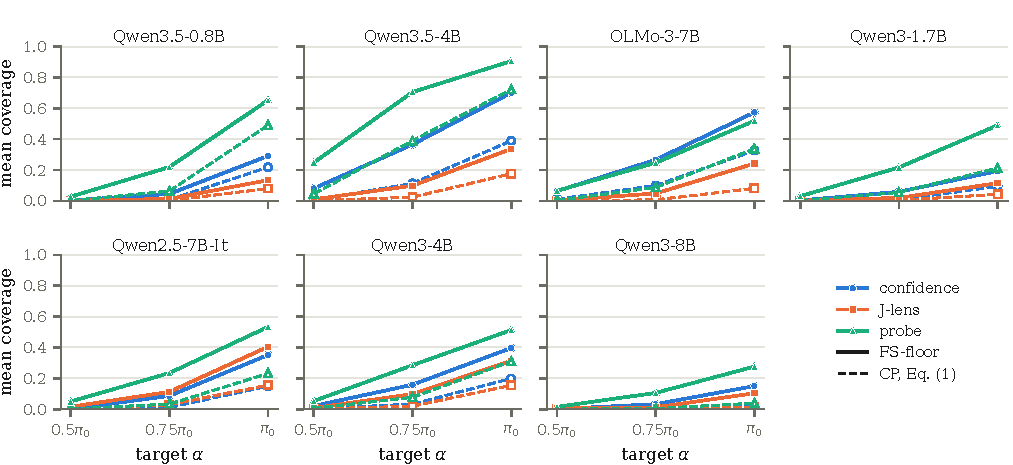
\includegraphics[width=\textwidth]{figs/fig_attain.pdf}
\caption{Mean coverage at the three relative targets for each model and principal signal on GSM8K: rule~\eqref{eq:cert} (dashed, open markers) and FS-floor with the cross-fitted grid and simulation-chosen $c$ (solid). FS-floor covers more in all 21 pairs at all three targets, and the gap is largest where the certificate fires at all.}
\label{fig:attain}
\end{figure}

\begin{figure}[H]
\centering
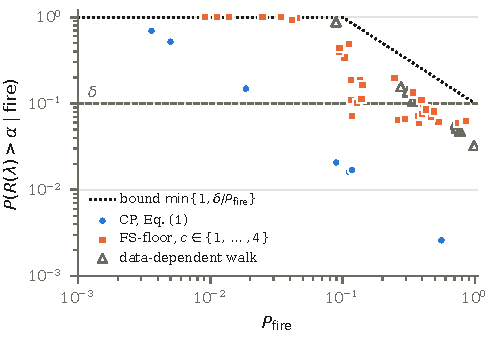
\includegraphics[width=0.5\textwidth]{figs/fig_abstention.pdf}
\caption{Validity by abstention in the Gaussian score model (the settings of Tables~\ref{tab:fs} and~\ref{tab:synthetic}). Each point is one procedure in one setting: the probability that an issued certificate is wrong, against the firing probability. Proposition~\ref{prop:abstain} bounds the former by $\min\{1,\delta/P_{\mathrm{fire}}\}$ (dotted). Rule~\eqref{eq:cert} sits far below $\delta$ where it fires often and far above it where it rarely fires; FS-floor sits near $\delta$; the data-dependent walk of \S\ref{sec:tighter} has no bound.}
\label{fig:abstention}
\end{figure}

\begin{figure}[H]
\centering
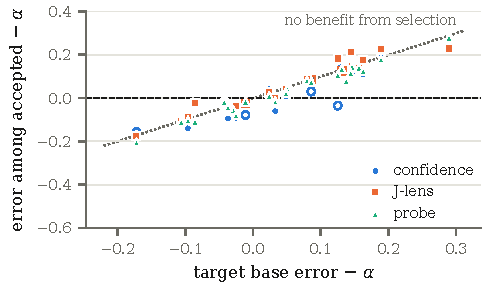
\includegraphics[width=0.55\textwidth]{figs/fig_shift.pdf}
\caption{GSM8K-calibrated certificates on other benchmarks (Section~\ref{sec:shift}; every cell in Table~\ref{tab:shift}): excess of the error among accepted traces over the target, against how much harder the new task is. Filled: mean coverage above $2\%$. On the dotted diagonal the accepted set is no better than accepting everything.}
\label{fig:shift}
\end{figure}

\begin{figure}[H]
\centering
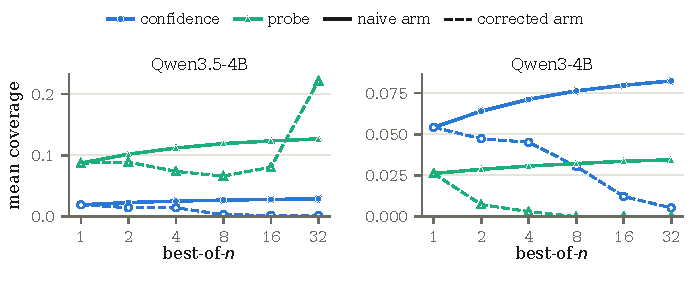
\includegraphics[width=0.68\textwidth]{figs/fig_corrected.pdf}
\caption{Best-of-$n$: mean coverage of the naive arm (solid; threshold calibrated on unpressured traces) and of the selection-conditional arm (dashed; calibration traces selected by the same best-of-$n$ rule), for the signals that fire in at least 2\% of replicates. The correction restores exchangeability, but its coverage collapses with $n$ except for the probe on Qwen3.5-4B, where best-of-$n$ lowers the policy's error below the target.}
\label{fig:corrected}
\end{figure}

\clearpage
\section{Additional Tables}
\label{app:exact}\label{app:auc}

\begin{table}[t]
\centering\small
\caption{Bounds in the same selective construction (same grid, Bonferroni split, data and replicates) at $\alpha=\pi_0$; 7 models $\times$ 3 signals. $^\dagger$No validity proof (see text).}
\label{tab:bounds}
\setlength{\tabcolsep}{4pt}
\begin{tabular}{lccc}
\toprule
Bound & Mean cov. & Cov.$\ge$10\% & Beats CP \\
\midrule
Clopper--Pearson & 0.211 & 14/21 & -- \\
Hoeffding--Bentkus & 0.156 & 12/21 & 0/21 \\
Betting mixture & 0.087 & 6/21 & 0/21 \\
\midrule
Data-dep.\ walk$^\dagger$ & 0.435 & 21/21 & -- \\
\bottomrule
\end{tabular}
\end{table}

\begin{table}[H]
\centering\small
\caption{Mean coverage of the CP certificate (in parentheses: $P_{\mathrm{fire}}$) for every model, target and signal; GSM8K, $\delta=0.10$, 1{,}000 replicates. ``Non-vac.'': target below the base error rate of the non-training problems.}
\label{tab:full}
\begin{tabular}{llrc ccccc}
\toprule
Model & Target & $\alpha$ & Non-vac. & Confidence & J-lens & Logit lens & Surface & Probe \\
\midrule
Qwen3.5-0.8B & $0.5\pi_0$ & 0.322 & yes & 0.000 (0.00) & 0.000 (0.00) & 0.000 (0.00) & 0.000 (0.00) & 0.002 (0.02) \\
 & $0.75\pi_0$ & 0.483 & yes & 0.007 (0.05) & 0.001 (0.01) & 0.000 (0.00) & 0.000 (0.00) & 0.063 (0.38) \\
 & $\pi_0$ & 0.644 & yes & 0.218 (0.58) & 0.080 (0.25) & 0.051 (0.13) & 0.000 (0.00) & 0.489 (0.96) \\
 & 0.05 & 0.050 & yes & 0.000 (0.00) & 0.000 (0.00) & 0.000 (0.00) & 0.000 (0.00) & 0.000 (0.00) \\
 & 0.10 & 0.100 & yes & 0.000 (0.00) & 0.000 (0.00) & 0.000 (0.00) & 0.000 (0.00) & 0.000 (0.00) \\
 & 0.20 & 0.200 & yes & 0.000 (0.00) & 0.000 (0.00) & 0.000 (0.00) & 0.000 (0.00) & 0.000 (0.00) \\
\addlinespace
Qwen3.5-4B & $0.5\pi_0$ & 0.081 & yes & 0.005 (0.01) & 0.000 (0.00) & 0.000 (0.00) & 0.000 (0.00) & 0.046 (0.08) \\
 & $0.75\pi_0$ & 0.122 & yes & 0.113 (0.22) & 0.024 (0.05) & 0.013 (0.03) & 0.001 (0.00) & 0.390 (0.62) \\
 & $\pi_0$ & 0.162 & no & 0.389 (0.57) & 0.176 (0.24) & 0.144 (0.21) & 0.054 (0.07) & 0.721 (0.93) \\
 & 0.05 & 0.050 & yes & 0.000 (0.00) & 0.000 (0.00) & 0.000 (0.00) & 0.000 (0.00) & 0.000 (0.00) \\
 & 0.10 & 0.100 & yes & 0.014 (0.03) & 0.002 (0.01) & 0.001 (0.00) & 0.000 (0.00) & 0.152 (0.28) \\
 & 0.20 & 0.200 & no & 0.727 (0.92) & 0.474 (0.61) & 0.427 (0.56) & 0.159 (0.19) & 0.898 (1.00) \\
\addlinespace
OLMo-3-7B & $0.5\pi_0$ & 0.172 & yes & 0.010 (0.02) & 0.000 (0.00) & 0.000 (0.00) & 0.000 (0.00) & 0.003 (0.01) \\
 & $0.75\pi_0$ & 0.258 & yes & 0.099 (0.19) & 0.007 (0.02) & 0.009 (0.02) & 0.003 (0.01) & 0.087 (0.21) \\
 & $\pi_0$ & 0.344 & no & 0.326 (0.53) & 0.081 (0.16) & 0.098 (0.15) & 0.086 (0.13) & 0.338 (0.54) \\
 & 0.05 & 0.050 & yes & 0.000 (0.00) & 0.000 (0.00) & 0.000 (0.00) & 0.000 (0.00) & 0.000 (0.00) \\
 & 0.10 & 0.100 & yes & 0.000 (0.00) & 0.000 (0.00) & 0.000 (0.00) & 0.000 (0.00) & 0.000 (0.00) \\
 & 0.20 & 0.200 & yes & 0.014 (0.03) & 0.000 (0.00) & 0.000 (0.00) & 0.000 (0.00) & 0.006 (0.02) \\
\addlinespace
Qwen3-1.7B & $0.5\pi_0$ & 0.107 & yes & 0.000 (0.00) & 0.000 (0.00) & 0.000 (0.00) & 0.000 (0.00) & 0.002 (0.00) \\
 & $0.75\pi_0$ & 0.160 & yes & 0.008 (0.01) & 0.003 (0.01) & 0.005 (0.01) & 0.004 (0.01) & 0.055 (0.09) \\
 & $\pi_0$ & 0.213 & yes & 0.094 (0.11) & 0.042 (0.05) & 0.082 (0.10) & 0.051 (0.07) & 0.212 (0.29) \\
 & 0.05 & 0.050 & yes & 0.000 (0.00) & 0.000 (0.00) & 0.000 (0.00) & 0.000 (0.00) & 0.000 (0.00) \\
 & 0.10 & 0.100 & yes & 0.000 (0.00) & 0.000 (0.00) & 0.000 (0.00) & 0.000 (0.00) & 0.000 (0.00) \\
 & 0.20 & 0.200 & yes & 0.023 (0.04) & 0.005 (0.01) & 0.006 (0.01) & 0.001 (0.00) & 0.131 (0.23) \\
\addlinespace
Qwen2.5-7B-It & $0.5\pi_0$ & 0.110 & yes & 0.000 (0.00) & 0.001 (0.00) & 0.000 (0.00) & 0.000 (0.00) & 0.001 (0.00) \\
 & $0.75\pi_0$ & 0.166 & yes & 0.012 (0.02) & 0.030 (0.06) & 0.016 (0.03) & 0.014 (0.02) & 0.033 (0.06) \\
 & $\pi_0$ & 0.221 & no & 0.149 (0.19) & 0.156 (0.24) & 0.118 (0.19) & 0.117 (0.14) & 0.232 (0.31) \\
 & 0.05 & 0.050 & yes & 0.000 (0.00) & 0.000 (0.00) & 0.000 (0.00) & 0.000 (0.00) & 0.000 (0.00) \\
 & 0.10 & 0.100 & yes & 0.000 (0.00) & 0.000 (0.00) & 0.000 (0.00) & 0.000 (0.00) & 0.000 (0.00) \\
 & 0.20 & 0.200 & no & 0.029 (0.04) & 0.064 (0.12) & 0.034 (0.06) & 0.023 (0.04) & 0.089 (0.15) \\
\addlinespace
Qwen3-4B & $0.5\pi_0$ & 0.051 & yes & 0.003 (0.00) & 0.001 (0.00) & 0.000 (0.00) & 0.000 (0.00) & 0.006 (0.01) \\
 & $0.75\pi_0$ & 0.076 & yes & 0.033 (0.05) & 0.019 (0.03) & 0.005 (0.01) & 0.011 (0.02) & 0.077 (0.11) \\
 & $\pi_0$ & 0.101 & no & 0.199 (0.25) & 0.155 (0.19) & 0.084 (0.10) & 0.109 (0.14) & 0.311 (0.39) \\
 & 0.05 & 0.050 & yes & 0.001 (0.00) & 0.000 (0.00) & 0.000 (0.00) & 0.000 (0.00) & 0.001 (0.00) \\
 & 0.10 & 0.100 & no & 0.064 (0.10) & 0.041 (0.06) & 0.008 (0.01) & 0.021 (0.03) & 0.123 (0.19) \\
 & 0.20 & 0.200 & no & 0.966 (0.99) & 0.942 (0.98) & 0.902 (0.92) & 0.928 (0.96) & 0.974 (0.99) \\
\addlinespace
Qwen3-8B & $0.5\pi_0$ & 0.047 & yes & 0.000 (0.00) & 0.000 (0.00) & 0.000 (0.00) & 0.000 (0.00) & 0.000 (0.00) \\
 & $0.75\pi_0$ & 0.071 & yes & 0.002 (0.00) & 0.001 (0.00) & 0.001 (0.00) & 0.001 (0.00) & 0.004 (0.01) \\
 & $\pi_0$ & 0.095 & no & 0.016 (0.02) & 0.014 (0.02) & 0.009 (0.01) & 0.004 (0.00) & 0.039 (0.05) \\
 & 0.05 & 0.050 & yes & 0.000 (0.00) & 0.000 (0.00) & 0.000 (0.00) & 0.000 (0.00) & 0.000 (0.00) \\
 & 0.10 & 0.100 & no & 0.007 (0.01) & 0.007 (0.01) & 0.004 (0.00) & 0.004 (0.00) & 0.025 (0.03) \\
 & 0.20 & 0.200 & no & 0.577 (0.65) & 0.488 (0.52) & 0.399 (0.43) & 0.385 (0.41) & 0.731 (0.80) \\
\bottomrule
\end{tabular}
\end{table}

\begin{table}[H]
\centering\small
\caption{Left: test AUC of the frozen scorer, and coverage of rule~\eqref{eq:cert} (``excl.'', boundary trace excluded) and of the boundary-included variant (``incl.''), $\alpha=\pi_0$. Right: BH conformal selection at level $\alpha=\pi_0$: mean number of calibration errors $n_0$, the lattice minimum $\lceil m/(\alpha(n_0+1))\rceil$ of Proposition~\ref{prop:lattice} relative to the test size $m$, and the fraction of replicates with no rejection.}
\label{tab:bh}
\setlength{\tabcolsep}{2.6pt}
\begin{tabular}{l ccc ccc ccc rr ccc}
\toprule
 & \multicolumn{3}{c}{Confidence} & \multicolumn{3}{c}{J-lens} & \multicolumn{3}{c}{Probe} & & & \multicolumn{3}{c}{BH: no rejection} \\
\cmidrule(lr){2-4}\cmidrule(lr){5-7}\cmidrule(lr){8-10}\cmidrule(lr){13-15}
Model & AUC & excl. & incl. & AUC & excl. & incl. & AUC & excl. & incl. & $n_0$ & min.\ rej. & Conf. & J-lens & Probe \\
\midrule
Qwen3.5-0.8B & 0.70 & 0.218 & 0.213 & 0.66 & 0.080 & 0.077 & 0.81 & 0.489 & 0.486 & 107.8 & 2/119 & 0.09 & 0.21 & 0.01 \\
Qwen3.5-4B & 0.73 & 0.389 & 0.390 & 0.65 & 0.176 & 0.172 & 0.82 & 0.721 & 0.715 & 23.4 & 31/116 & 0.87 & 0.97 & 0.57 \\
OLMo-3-7B & 0.75 & 0.326 & 0.313 & 0.63 & 0.081 & 0.081 & 0.76 & 0.338 & 0.323 & 23.4 & 6/50 & 0.41 & 0.69 & 0.28 \\
Qwen3-1.7B & 0.66 & 0.094 & 0.088 & 0.61 & 0.042 & 0.047 & 0.76 & 0.212 & 0.216 & 17.9 & 15/58 & 0.96 & 0.96 & 0.76 \\
Qwen2.5-7B-It & 0.60 & 0.149 & 0.160 & 0.62 & 0.156 & 0.157 & 0.68 & 0.232 & 0.232 & 12.9 & 18/54 & 0.98 & 0.90 & 0.91 \\
Qwen3-4B & 0.66 & 0.199 & 0.189 & 0.61 & 0.155 & 0.148 & 0.71 & 0.311 & 0.300 & 14.3 & 79/114 & 1.00 & 1.00 & 1.00 \\
Qwen3-8B & 0.61 & 0.016 & 0.019 & 0.47 & 0.014 & 0.012 & 0.67 & 0.039 & 0.043 & 6.5 & 79/55 & 1.00 & 1.00 & 1.00 \\
\bottomrule
\end{tabular}
\end{table}

\begin{table}[H]
\centering\small
\caption{Gaussian score model with known selective risk; 20{,}000 calibration draws per row, $\delta=0.10$. $P(R>\alpha)$ is the quantity bounded by $(\alpha,\delta)$-validity; $P(R>\alpha\mid\text{fire})$ is the probability that an issued certificate is wrong; the next two columns give the median and 90th percentile of $R(\hat\lambda)/\alpha$ among failing draws, i.e.\ how far a wrong certificate overshoots its target.}
\label{tab:synthetic}
\setlength{\tabcolsep}{4pt}
\begin{tabular}{cccc l cccccc}
\toprule
$\pi_0$ & AUC & $n_{\mathrm{cal}}$ & $\alpha$ & Procedure & $P_{\mathrm{fire}}$ & $P(R>\alpha)$ & $P(R>\alpha\mid\text{fire})$ & med.\ $R/\alpha$ & p90 $R/\alpha$ & Mean cov. \\
\midrule
0.16 & 0.82 & 154 & $0.75\pi_0$ & CP, Eq.~(1) & 0.558 & 0.0014 & 0.003 & 1.06 & 1.13 & 0.322 \\
0.16 & 0.82 & 154 & $0.75\pi_0$ & Data-dep.\ walk & 0.985 & 0.0319 & 0.032 & 1.06 & 1.24 & 0.631 \\
\addlinespace
0.16 & 0.82 & 154 & $0.5\pi_0$ & CP, Eq.~(1) & 0.089 & 0.0019 & 0.021 & 1.04 & 1.15 & 0.049 \\
0.16 & 0.82 & 154 & $0.5\pi_0$ & Data-dep.\ walk & 0.770 & 0.0368 & 0.048 & 1.11 & 1.34 & 0.331 \\
\addlinespace
0.16 & 0.71 & 154 & $0.75\pi_0$ & CP, Eq.~(1) & 0.112 & 0.0018 & 0.016 & 1.04 & 1.14 & 0.054 \\
0.16 & 0.71 & 154 & $0.75\pi_0$ & Data-dep.\ walk & 0.724 & 0.0374 & 0.052 & 1.09 & 1.20 & 0.306 \\
\addlinespace
0.16 & 0.71 & 154 & $0.5\pi_0$ & CP, Eq.~(1) & 0.005 & 0.0026 & 0.520 & 1.12 & 1.28 & 0.003 \\
0.16 & 0.71 & 154 & $0.5\pi_0$ & Data-dep.\ walk & 0.276 & 0.0433 & 0.157 & 1.11 & 1.35 & 0.092 \\
\addlinespace
0.22 & 0.76 & 78 & $0.75\pi_0$ & CP, Eq.~(1) & 0.118 & 0.0020 & 0.017 & 1.07 & 1.22 & 0.061 \\
0.22 & 0.76 & 78 & $0.75\pi_0$ & Data-dep.\ walk & 0.712 & 0.0411 & 0.058 & 1.10 & 1.27 & 0.339 \\
\addlinespace
0.22 & 0.76 & 78 & $0.5\pi_0$ & CP, Eq.~(1) & 0.004 & 0.0025 & 0.694 & 1.11 & 1.23 & 0.002 \\
0.22 & 0.76 & 78 & $0.5\pi_0$ & Data-dep.\ walk & 0.309 & 0.0418 & 0.135 & 1.14 & 1.40 & 0.135 \\
\addlinespace
0.09 & 0.66 & 153 & $0.75\pi_0$ & CP, Eq.~(1) & 0.019 & 0.0027 & 0.148 & 1.12 & 1.24 & 0.011 \\
0.09 & 0.66 & 153 & $0.75\pi_0$ & Data-dep.\ walk & 0.337 & 0.0359 & 0.106 & 1.11 & 1.27 & 0.158 \\
\addlinespace
0.09 & 0.66 & 153 & $0.5\pi_0$ & CP, Eq.~(1) & 0.000 & 0.0001 & 1.000 & 1.59 & 1.62 & 0.000 \\
0.09 & 0.66 & 153 & $0.5\pi_0$ & Data-dep.\ walk & 0.089 & 0.0786 & 0.882 & 1.11 & 1.37 & 0.041 \\
\bottomrule
\end{tabular}
\end{table}

\begin{table}[H]
\centering\scriptsize
\caption{FS-floor on real data, mean coverage for each (model, signal) pair; GSM8K, $\delta=0.10$, 1{,}000 replicates. CP: rule~\eqref{eq:cert}. In-s.: FS-floor with the grid from in-sample training scores, $c=2$. $c{=}1,\dots,4$: cross-fitted grid at fixed $c$. Sim.: cross-fitted grid with $c$ chosen per cell by the pre-calibration simulation.}
\label{tab:fsfull}
\setlength{\tabcolsep}{2.2pt}
\begin{tabular}{ll cccccccc cccccccc}
\toprule
 & & \multicolumn{8}{c}{$\alpha=\pi_0$} & \multicolumn{8}{c}{$\alpha=0.75\pi_0$} \\
\cmidrule(lr){3-10}\cmidrule(lr){11-18}
Model & Signal & CP & In-s. & $c{=}1$ & $1.5$ & $2$ & $3$ & $4$ & Sim. & CP & In-s. & $c{=}1$ & $1.5$ & $2$ & $3$ & $4$ & Sim. \\
\midrule
Qwen3.5-0.8B & Conf. & 0.218 & 0.113 & 0.037 & 0.134 & 0.134 & 0.217 & 0.291 & 0.291 & 0.007 & 0.023 & 0.012 & 0.012 & 0.021 & 0.034 & 0.043 & 0.045 \\
 & J-lens & 0.080 & 0.076 & 0.007 & 0.030 & 0.030 & 0.094 & 0.134 & 0.134 & 0.001 & 0.011 & 0.002 & 0.002 & 0.007 & 0.011 & 0.013 & 0.013 \\
 & Probe & 0.489 & 0.278 & 0.319 & 0.502 & 0.502 & 0.616 & 0.652 & 0.652 & 0.063 & 0.064 & 0.108 & 0.108 & 0.151 & 0.180 & 0.219 & 0.219 \\
\addlinespace
Qwen3.5-4B & Conf. & 0.389 & 0.466 & 0.241 & 0.367 & 0.464 & 0.650 & 0.701 & 0.701 & 0.113 & 0.280 & 0.131 & 0.194 & 0.253 & 0.366 & 0.313 & 0.365 \\
 & J-lens & 0.176 & 0.223 & 0.018 & 0.100 & 0.166 & 0.269 & 0.336 & 0.336 & 0.024 & 0.074 & 0.014 & 0.045 & 0.067 & 0.091 & 0.097 & 0.098 \\
 & Probe & 0.721 & 0.736 & 0.481 & 0.719 & 0.822 & 0.893 & 0.905 & 0.905 & 0.390 & 0.544 & 0.362 & 0.517 & 0.644 & 0.699 & 0.705 & 0.705 \\
\addlinespace
OLMo-3-7B & Conf. & 0.326 & 0.424 & 0.056 & 0.251 & 0.378 & 0.543 & 0.573 & 0.573 & 0.099 & 0.220 & 0.046 & 0.122 & 0.218 & 0.268 & 0.259 & 0.266 \\
 & J-lens & 0.081 & 0.198 & 0.021 & 0.058 & 0.102 & 0.177 & 0.242 & 0.242 & 0.007 & 0.048 & 0.007 & 0.018 & 0.022 & 0.058 & 0.072 & 0.048 \\
 & Probe & 0.338 & 0.116 & 0.307 & 0.467 & 0.497 & 0.538 & 0.518 & 0.518 & 0.087 & 0.050 & 0.210 & 0.237 & 0.256 & 0.246 & 0.264 & 0.246 \\
\addlinespace
Qwen3-1.7B & Conf. & 0.094 & 0.071 & 0.043 & 0.057 & 0.078 & 0.167 & 0.193 & 0.193 & 0.008 & 0.020 & 0.010 & 0.013 & 0.024 & 0.060 & 0.058 & 0.059 \\
 & J-lens & 0.042 & 0.090 & 0.044 & 0.058 & 0.070 & 0.093 & 0.115 & 0.115 & 0.003 & 0.023 & 0.013 & 0.015 & 0.020 & 0.018 & 0.019 & 0.019 \\
 & Probe & 0.212 & 0.140 & 0.169 & 0.195 & 0.262 & 0.411 & 0.454 & 0.489 & 0.055 & 0.050 & 0.055 & 0.107 & 0.130 & 0.174 & 0.170 & 0.216 \\
\addlinespace
Qwen2.5-7B-It & Conf. & 0.149 & 0.219 & 0.039 & 0.058 & 0.171 & 0.236 & 0.352 & 0.352 & 0.012 & 0.071 & 0.008 & 0.033 & 0.049 & 0.124 & 0.088 & 0.086 \\
 & J-lens & 0.156 & 0.349 & 0.184 & 0.260 & 0.329 & 0.405 & 0.403 & 0.405 & 0.030 & 0.140 & 0.073 & 0.115 & 0.142 & 0.125 & 0.067 & 0.112 \\
 & Probe & 0.232 & 0.104 & 0.206 & 0.295 & 0.363 & 0.493 & 0.522 & 0.533 & 0.033 & 0.049 & 0.076 & 0.104 & 0.180 & 0.231 & 0.155 & 0.234 \\
\addlinespace
Qwen3-4B & Conf. & 0.199 & 0.283 & 0.025 & 0.143 & 0.274 & 0.375 & 0.391 & 0.396 & 0.033 & 0.132 & 0.010 & 0.079 & 0.121 & 0.168 & 0.181 & 0.159 \\
 & J-lens & 0.155 & 0.240 & 0.086 & 0.172 & 0.200 & 0.244 & 0.311 & 0.314 & 0.019 & 0.077 & 0.048 & 0.054 & 0.071 & 0.103 & 0.124 & 0.098 \\
 & Probe & 0.311 & 0.403 & 0.241 & 0.340 & 0.457 & 0.482 & 0.508 & 0.513 & 0.077 & 0.197 & 0.107 & 0.189 & 0.237 & 0.285 & 0.285 & 0.285 \\
\addlinespace
Qwen3-8B & Conf. & 0.016 & 0.108 & 0.027 & 0.109 & 0.116 & 0.155 & 0.000 & 0.150 & 0.002 & 0.047 & 0.023 & 0.030 & 0.039 & 0.000 & 0.000 & 0.033 \\
 & J-lens & 0.014 & 0.106 & 0.015 & 0.056 & 0.090 & 0.089 & 0.000 & 0.104 & 0.001 & 0.012 & 0.017 & 0.033 & 0.012 & 0.000 & 0.000 & 0.012 \\
 & Probe & 0.039 & 0.139 & 0.146 & 0.180 & 0.238 & 0.269 & 0.000 & 0.276 & 0.004 & 0.068 & 0.076 & 0.075 & 0.101 & 0.000 & 0.000 & 0.106 \\
\bottomrule
\end{tabular}
\end{table}

\begin{table}[H]
\centering\scriptsize
\caption{Every shift cell (Section~\ref{sec:shift}): GSM8K-trained scorer and GSM8K-calibrated threshold ($\alpha$: training-partition base error on GSM8K) applied to the same model's traces on another benchmark. $\pi_{\mathrm{new}}$: base error rate on the new benchmark. Per signal: mean coverage and $\hat R$, the error among accepted traces pooled over firing replicates; bold where $\hat R>\alpha$. 1{,}000 replicates per cell.}
\label{tab:shift}
\setlength{\tabcolsep}{4pt}
\begin{tabular}{ll cc cc cc cc}
\toprule
 & & & & \multicolumn{2}{c}{Confidence} & \multicolumn{2}{c}{J-lens} & \multicolumn{2}{c}{Probe} \\
\cmidrule(lr){5-6}\cmidrule(lr){7-8}\cmidrule(lr){9-10}
Model & Benchmark & $\pi_{\mathrm{new}}$ & $\alpha$ & Cov. & $\hat R$ & Cov. & $\hat R$ & Cov. & $\hat R$ \\
\midrule
Qwen3.5-0.8B & ARC-C & 0.77 & 0.64 & 0.00 & 0.61 & 0.06 & \textbf{0.83} & 0.27 & \textbf{0.75} \\
 & BBH-logic & 0.61 & 0.64 & 0.07 & 0.55 & 0.05 & 0.59 & 0.09 & 0.60 \\
 & CSQA & 0.79 & 0.64 & 0.00 & 0.01 & 0.05 & \textbf{0.86} & 0.27 & \textbf{0.76} \\
 & StrategyQA & 0.47 & 0.64 & 0.00 & 0.49 & 0.10 & 0.47 & 0.13 & 0.44 \\
\addlinespace
Qwen3.5-4B & ARC-C & 0.07 & 0.16 & 0.11 & 0.02 & 0.27 & 0.07 & 0.60 & 0.06 \\
 & BBH-logic & 0.19 & 0.16 & 0.29 & \textbf{0.20} & 0.28 & \textbf{0.19} & 0.60 & \textbf{0.17} \\
 & CSQA & 0.20 & 0.16 & 0.05 & 0.10 & 0.23 & 0.16 & 0.52 & 0.15 \\
 & StrategyQA & 0.33 & 0.16 & 0.09 & \textbf{0.27} & 0.23 & \textbf{0.34} & 0.59 & \textbf{0.29} \\
\addlinespace
OLMo-3-7B & ARC-C & 0.26 & 0.34 & 0.21 & 0.22 & 0.09 & 0.32 & 0.44 & 0.24 \\
 & BBH-logic & 0.63 & 0.34 & 0.44 & \textbf{0.60} & 0.07 & \textbf{0.57} & 0.35 & \textbf{0.62} \\
 & CSQA & 0.30 & 0.34 & 0.20 & 0.33 & 0.06 & 0.32 & 0.52 & 0.33 \\
\addlinespace
Qwen3-1.7B & ARC-C & 0.19 & 0.21 & 0.09 & 0.12 & 0.14 & 0.18 & 0.11 & 0.13 \\
 & CSQA & 0.35 & 0.21 & 0.10 & \textbf{0.29} & 0.14 & \textbf{0.35} & 0.10 & \textbf{0.29} \\
 & StrategyQA & 0.36 & 0.21 & 0.04 & \textbf{0.32} & 0.14 & \textbf{0.36} & 0.06 & \textbf{0.36} \\
\addlinespace
Qwen2.5-7B-It & ARC-C & 0.11 & 0.22 & 0.34 & 0.12 & 0.41 & 0.12 & 0.35 & 0.11 \\
 & BBH-logic & 0.41 & 0.22 & 0.33 & \textbf{0.42} & 0.42 & \textbf{0.45} & 0.39 & \textbf{0.40} \\
 & CSQA & 0.19 & 0.22 & 0.35 & 0.17 & 0.43 & 0.16 & 0.41 & 0.17 \\
 & StrategyQA & 0.27 & 0.22 & 0.34 & \textbf{0.26} & 0.37 & \textbf{0.25} & 0.42 & \textbf{0.26} \\
\addlinespace
Qwen3-4B & ARC-C & 0.15 & 0.10 & 0.31 & \textbf{0.11} & 0.29 & \textbf{0.14} & 0.37 & \textbf{0.12} \\
 & BBH-logic & 0.18 & 0.10 & 0.36 & \textbf{0.18} & 0.27 & \textbf{0.19} & 0.42 & \textbf{0.18} \\
 & StrategyQA & 0.26 & 0.10 & 0.27 & \textbf{0.23} & 0.32 & \textbf{0.24} & 0.30 & \textbf{0.24} \\
\addlinespace
Qwen3-8B & ARC-C & 0.08 & 0.09 & 0.02 & 0.02 & 0.01 & 0.07 & 0.10 & 0.08 \\
 & CSQA & 0.18 & 0.09 & 0.01 & \textbf{0.12} & 0.01 & \textbf{0.18} & 0.08 & \textbf{0.17} \\
 & StrategyQA & 0.23 & 0.09 & 0.02 & \textbf{0.23} & 0.01 & \textbf{0.22} & 0.13 & \textbf{0.23} \\
\bottomrule
\end{tabular}
\end{table}

\begin{table}[H]
\centering\scriptsize
\caption{Best-of-$n$ selection (Section~\ref{sec:pressure}) per model and signal. $P_{\mathrm{fire}}$: firing probability of the naive arm (independent of $n$). $\hat R/\alpha$: error among accepted BoN-selected test traces relative to the target, naive arm (-- where fewer than 2\% of replicates fire). Corrected: mean coverage of the selection-conditional arm at $n=1$ and $n=32$. $\Delta$acc: change in accuracy of the selected trace from $n=1$ to $n=32$, and from its peak over $n$ to $n=32$.}
\label{tab:bon}
\setlength{\tabcolsep}{4pt}
\begin{tabular}{ll c ccc cc cc}
\toprule
 & & & \multicolumn{3}{c}{$\hat R/\alpha$, naive} & \multicolumn{2}{c}{Corrected cov.} & \multicolumn{2}{c}{$\Delta$acc} \\
\cmidrule(lr){4-6}\cmidrule(lr){7-8}\cmidrule(lr){9-10}
Model & Signal & $P_{\mathrm{fire}}$ & $n{=}1$ & $n{=}8$ & $n{=}32$ & $n{=}1$ & $n{=}32$ & $n{=}32$ & from peak \\
\midrule
Qwen3.5-4B & confidence & 0.031 & 0.92 & 1.14 & 1.25 & 0.019 & 0.002 & -0.004 & -0.022 \\
 & J-lens & 0.015 & -- & -- & -- & 0.008 & 0.000 & +0.001 & -0.016 \\
 & probe & 0.136 & 0.70 & 0.89 & 0.69 & 0.087 & 0.222 & +0.038 & +0.000 \\
 & logit lens & 0.014 & -- & -- & -- & 0.008 & 0.000 & -0.017 & -0.032 \\
 & surface & 0.002 & -- & -- & -- & 0.001 & 0.000 & -0.040 & -0.040 \\
\addlinespace
Qwen3-4B & confidence & 0.093 & 0.78 & 0.91 & 1.12 & 0.054 & 0.005 & +0.001 & -0.006 \\
 & J-lens & 0.007 & -- & -- & -- & 0.006 & 0.000 & +0.005 & -0.005 \\
 & probe & 0.045 & 0.87 & 1.33 & 1.52 & 0.026 & 0.000 & -0.029 & -0.031 \\
 & logit lens & 0.008 & -- & -- & -- & 0.004 & 0.000 & -0.001 & -0.003 \\
 & surface & 0.007 & -- & -- & -- & 0.005 & 0.000 & -0.017 & -0.017 \\
\bottomrule
\end{tabular}
\end{table}

\begin{table}[H]
\centering\small
\caption{GSM8K out-of-fold AUC (5-fold, grouped by problem, logistic regression) of each signal, and paired bootstrap differences ($^{*}$: two-sided $p<0.05$, uncorrected). ``Random'': J-lens features with a norm-matched random transport. These are cross-validated AUCs on all traces and differ from the frozen-scorer test AUCs of Table~\ref{tab:main}.}
\label{tab:auc}
\setlength{\tabcolsep}{4pt}
\begin{tabular}{lrr cccccc ccc}
\toprule
Model & Traces & Acc. & Conf. & J-lens & Logit lens & Surface & Random & Probe & J$-$Conf. & J$-$Surf. & Probe$-$J \\
\midrule
Qwen3.5-0.8B & 1244 & 0.33 & 0.714 & 0.713 & 0.661 & 0.531 & 0.641 & 0.842 & -0.001 & +0.182$^{*}$ & +0.129$^{*}$ \\
Qwen3.5-4B & 1365 & 0.84 & 0.715 & 0.707 & 0.669 & 0.515 & 0.553 & 0.847 & -0.009 & +0.191$^{*}$ & +0.140$^{*}$ \\
OLMo-3-7B & 295 & 0.66 & 0.748 & 0.642 & 0.595 & 0.613 & 0.594 & 0.770 & -0.106$^{*}$ & +0.029 & +0.128$^{*}$ \\
Qwen3-1.7B & 373 & 0.78 & 0.675 & 0.679 & 0.635 & 0.612 & 0.604 & 0.810 & +0.005 & +0.067 & +0.131$^{*}$ \\
Qwen2.5-7B-It & 323 & 0.81 & 0.584 & 0.648 & 0.522 & 0.602 & 0.559 & 0.668 & +0.065 & +0.046 & +0.020 \\
Qwen3-4B & 1387 & 0.91 & 0.610 & 0.607 & 0.551 & 0.549 & 0.625 & 0.751 & -0.003 & +0.057 & +0.144$^{*}$ \\
Qwen3-8B & 350 & 0.91 & 0.592 & 0.344 & 0.411 & 0.271 & 0.479 & 0.809 & -0.248$^{*}$ & +0.073 & +0.466$^{*}$ \\
\bottomrule
\end{tabular}
\end{table}

